\documentclass[twoside]{book}

% Packages required by doxygen
\usepackage{fixltx2e}
\usepackage{calc}
\usepackage{doxygen}
\usepackage[export]{adjustbox} % also loads graphicx
\usepackage{graphicx}
\usepackage[utf8]{inputenc}
\usepackage{makeidx}
\usepackage{multicol}
\usepackage{multirow}
\PassOptionsToPackage{warn}{textcomp}
\usepackage{textcomp}
\usepackage[nointegrals]{wasysym}
\usepackage[table]{xcolor}

% Font selection
\usepackage[T1]{fontenc}
\usepackage[scaled=.90]{helvet}
\usepackage{courier}
\usepackage{amssymb}
\usepackage{sectsty}
\renewcommand{\familydefault}{\sfdefault}
\allsectionsfont{%
  \fontseries{bc}\selectfont%
  \color{darkgray}%
}
\renewcommand{\DoxyLabelFont}{%
  \fontseries{bc}\selectfont%
  \color{darkgray}%
}
\newcommand{\+}{\discretionary{\mbox{\scriptsize$\hookleftarrow$}}{}{}}

% Page & text layout
\usepackage{geometry}
\geometry{%
  a4paper,%
  top=2.5cm,%
  bottom=2.5cm,%
  left=2.5cm,%
  right=2.5cm%
}
\tolerance=750
\hfuzz=15pt
\hbadness=750
\setlength{\emergencystretch}{15pt}
\setlength{\parindent}{0cm}
\setlength{\parskip}{3ex plus 2ex minus 2ex}
\makeatletter
\renewcommand{\paragraph}{%
  \@startsection{paragraph}{4}{0ex}{-1.0ex}{1.0ex}{%
    \normalfont\normalsize\bfseries\SS@parafont%
  }%
}
\renewcommand{\subparagraph}{%
  \@startsection{subparagraph}{5}{0ex}{-1.0ex}{1.0ex}{%
    \normalfont\normalsize\bfseries\SS@subparafont%
  }%
}
\makeatother

% Headers & footers
\usepackage{fancyhdr}
\pagestyle{fancyplain}
\fancyhead[LE]{\fancyplain{}{\bfseries\thepage}}
\fancyhead[CE]{\fancyplain{}{}}
\fancyhead[RE]{\fancyplain{}{\bfseries\leftmark}}
\fancyhead[LO]{\fancyplain{}{\bfseries\rightmark}}
\fancyhead[CO]{\fancyplain{}{}}
\fancyhead[RO]{\fancyplain{}{\bfseries\thepage}}
\fancyfoot[LE]{\fancyplain{}{}}
\fancyfoot[CE]{\fancyplain{}{}}
\fancyfoot[RE]{\fancyplain{}{\bfseries\scriptsize Generated by Doxygen }}
\fancyfoot[LO]{\fancyplain{}{\bfseries\scriptsize Generated by Doxygen }}
\fancyfoot[CO]{\fancyplain{}{}}
\fancyfoot[RO]{\fancyplain{}{}}
\renewcommand{\footrulewidth}{0.4pt}
\renewcommand{\chaptermark}[1]{%
  \markboth{#1}{}%
}
\renewcommand{\sectionmark}[1]{%
  \markright{\thesection\ #1}%
}

% Indices & bibliography
\usepackage{natbib}
\usepackage[titles]{tocloft}
\setcounter{tocdepth}{3}
\setcounter{secnumdepth}{5}
\makeindex

% Hyperlinks (required, but should be loaded last)
\usepackage{ifpdf}
\ifpdf
  \usepackage[pdftex,pagebackref=true]{hyperref}
\else
  \usepackage[ps2pdf,pagebackref=true]{hyperref}
\fi
\hypersetup{%
  colorlinks=true,%
  linkcolor=blue,%
  citecolor=blue,%
  unicode%
}

% Custom commands
\newcommand{\clearemptydoublepage}{%
  \newpage{\pagestyle{empty}\cleardoublepage}%
}

\usepackage{caption}
\captionsetup{labelsep=space,justification=centering,font={bf},singlelinecheck=off,skip=4pt,position=top}

%===== C O N T E N T S =====

\begin{document}

% Titlepage & ToC
\hypersetup{pageanchor=false,
             bookmarksnumbered=true,
             pdfencoding=unicode
            }
\pagenumbering{roman}
\begin{titlepage}
\vspace*{7cm}
\begin{center}%
{\Large rsync\+F\+TP \\[1ex]\large 1.\+2 }\\
\vspace*{1cm}
{\large Athors : Julien Vermeil, Nicolas Sobczak, Vincent Reynaert}\\
\vspace{3\baselineskip}
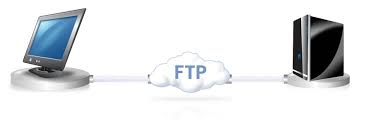
\includegraphics{../image.jpg}
\end{center}
\end{titlepage}
\clearemptydoublepage
\tableofcontents
\clearemptydoublepage
\pagenumbering{arabic}
\hypersetup{pageanchor=true}

%--- Begin generated contents ---
\chapter{Présentation}
\textit{rsyncFTP} est un programme permettant de créer un dossier miroir sur un serveur ftp distant.\\
\\
Le principe de ce programme est de mettre à jour le dossier situé sur le serveur distant en fonction de l'état du dossier 
situé en local une machine. Pour synchoniser ce fichier, il faut surveiller le dossier local et 
réaliser les actions nécessaires à la mise à jour du dossier miroir.\\
\\
Ce programme a été réalisé en python. La version utilisée est la version 3.5.2.
\chapter{Choix d'organisation}
Nous avons voulu séparer le plus possible les fonctionnalités en créant des fichiers différents: 
\begin{itemize}
\item logger.py
\item parser.py
\item gestionFTP.py
\item directorySupervisor.py
\item main.py
\end{itemize}

\section{logger.py}	

Le package logger contient la gestion du logger. C'est ici qu'on s'occupe de créer le logger.

\section{parser.py}

Le package parser contient la fonction de définition de gestion du parser. 
C'est ici que nous définissons les paramètres que nous passons en lignes de commandes.

\section{gestionFTP.py}

Le package gestionFTP contient toutes les fonctions utiles pour gérer les actions basiques avec le serveur FTP.

\section{directorySupervisor.py}

Le package directorySupervisor correspond à la supervision des dossiers. 
Il s'agit des fonctions du tp1 que nous avons adaptées pour rsyncFTP. 
Nous n'en avons repris que le coeur de façon a garder une certaine souplesse par rapport àa ce que nous avions déjà réalisé.
C'est à dire que nous l'avons amélioré notamment en supprimant les variables globales qui était dangereuses.

\section{main.py}

Le package main contient les fonctions principales. 
Nous avons chercher à le réduire à l'essentiel de façon à ce qu'il reste lisible et compréhensible au premier coup d'oeil.\\
\\
Les quelques étapes que nous réalisons sont les suivantes :
\begin{itemize}
\item Nous définissons notre parser.
\item Nous initialisons le logger.
\item Nous lançons ensuite notre boucle principale qui supervise le dossier et synchornise le répertoire situé sur le serveur FTP distant.
\end{itemize}

\chapter{Choix techniques}
La version de python utilisée est la 3.5.2. 
Le programme a été testé sur avec les serveurs FTP :
\begin{itemize}
\item \textit{Filezilla} (version ..) pour windows
\item \textit{Proftpd} pour linux, avec son interface graphique Gadmin ProFTPD (version 0.4.2)
\end{itemize}

\section{Synchronisation}
Pour synchroniser le dossier miroir, nous avons choisi de surveiller notre dossier local et alors de mettre à jour le dossier miroir.

\section{Paramètres}	

\newcolumntype{R}[1]{>{\raggedleft\arraybackslash }b{#1}}
\newcolumntype{L}[1]{>{\raggedright\arraybackslash }b{#1}}
\newcolumntype{C}[1]{>{\centering\arraybackslash }b{#1}}

Nous avons choisi de passer en ligne de commande les paramètres suivants:

\begin{tabular}{|R{8cm}|C{3cm}|L{3cm}|}
\hline \rowcolor{lightgray} Paramètre & Type &  Variable  \\
\hline  site ftp distant & obligatoire & ftp  \\
\hline  chemin vers le dossier local (directory path) & obligatoire & dp  \\
\hline  chemin pour generer le fichier log (log path) & obligatoire & lp  \\
\hline  2-uple contenant les extensions de la liste de fichiers a inclure et de la liste de fichiers a exclure & obligatoire & ie  \\
\hline  chemin vers le fichier conf du log (gestion des handler) & optionnel & "-lc", "--logConf"  \\
\hline  profondeur de la supervision du dossier, default = 2 & optionnel & "-p", "--profondeur"  \\
\hline  taille maximale des fichiers transferes en Mo, default = 500 Mo & optionnel & "-sf","--sizeFile"  \\
\hline  frequence de supervision en s, default = 1 s & optionnel & "-f", "--frequence"  \\
\hline  temps de supervision en s, default = 60 sec & optionnel & "-st", "--supervisionTime"  \\

\hline 
\end{tabular}

\section{Fichier log}

Concernant le fichier de log, si aucun chemin pour enregistrer le fichier n'est précisé, nous utilisons le fichier .conf qui nous définit des handlers proprement et enregistre le fichier log dans le répertoire du projet.
Si un chemin est précisé, nous n'utilisons pas le fichier log. Nous créons le logger dans le code du fichier logger.py. Le fichier rsyncFTP.log est alors enregistré dans le répertoire précisé par le chemin entré en ligne de commande.


\section{Librairie gestionFTP}

Dans la librairie \textit{gestionFTP}, nous avons choisi de définir des fonctions permettant de réaliser des actions basiques telles que : 
\begin{itemize}
\item créer un fichier sur le seveur ftp
\item transferer un fichier vers le seveur ftp
\item effacer un fichier sur le seveur ftp
\item créer un dossier sur le seveur ftp
\item transferer un dossier vers le seveur ftp
\item effacer un dossier sur le seveur ftp
\end{itemize}

Nous pouvons alors executer ces actions pour réaliser des fonctions plus complexes.\\
\\
Nous avons rencontré une difficulté concernant la fonction qui supprime un dossier. 
Elle est un peu similaire à celle qui copie un dossier à ceci près qu'elle que l'on rencontre un probleme lorsque l'on
veut supprimer un dossier ou un fichier car il n'existe plus en local. On ne peut donc pas vérifier si ce 
qu'on veut supprimer sur le serveur ftp est un fichier ou un dossier. En outre, pour supprimer un dossier, nous devons en supprimer 
tout son contenu. Il nous a donc fallu créer une fonction récursive pour vider les dossiers avant de les supprimer.


\section{Librairie directorySupervisor}

Pour pouvoir superviser un dossier, nous utilisons l'organisation des répertoire en ``arbre``.
Nous avons choisi de ne pas créer de classe arbre mais plutôt de matérialiser un arbre avec une liste.\\
\\
Nous créons donc d'abord l'arbre du dossier à chaque fois qu'il s'écoule une période correspondant à la fréquence de supervision. 
Puis nous comparons cette arbre avec l'arbre précédemment créé. 
Si on observe une modification, on l'écrit dans le fichier de log et on va signaler le type de modification effectuée afin de pouvoir mettre à jour le dossier situé sur le serveur distant.\\
\\





\chapter{Namespace Index}
\section{Packages}
Here are the packages with brief descriptions (if available)\+:\begin{DoxyCompactList}
\item\contentsline{section}{\hyperlink{namespacedirectory_supervisor}{directory\+Supervisor} }{\pageref{namespacedirectory_supervisor}}{}
\item\contentsline{section}{\hyperlink{namespacegestion_f_t_p}{gestion\+F\+TP} }{\pageref{namespacegestion_f_t_p}}{}
\item\contentsline{section}{\hyperlink{namespacemain}{main} }{\pageref{namespacemain}}{}
\item\contentsline{section}{\hyperlink{namespaceparser_rsync_f_t_p}{parser\+Rsync\+F\+TP} }{\pageref{namespaceparser_rsync_f_t_p}}{}
\end{DoxyCompactList}

\chapter{Namespace Documentation}
\hypertarget{namespacedirectory_supervisor}{}\section{directory\+Supervisor Namespace Reference}
\label{namespacedirectory_supervisor}\index{directory\+Supervisor@{directory\+Supervisor}}
\subsection*{Functions}
\begin{DoxyCompactItemize}
\item 
def \hyperlink{namespacedirectory_supervisor_a9d74cc8524cb7e3e77edb67c0ee845ca}{create\+Survey\+List} (tree, startinglevel, depth)
\item 
def \hyperlink{namespacedirectory_supervisor_a8320472c590edd49c3dece24e50f0751}{comparate\+Survey\+List} (old\+Liste, new\+Liste)
\item 
def \hyperlink{namespacedirectory_supervisor_a318858380e4893dce2f9d4a878c954c9}{log\+The\+M\+A\+D\+Lists} (logger, M, A, D)
\item 
def \hyperlink{namespacedirectory_supervisor_a79c093888347915f7624fbac8f61e0be}{loop} (logger, frequence, supervision\+Time, arbre\+Precedent, dp)
\item 
def \hyperlink{namespacedirectory_supervisor_a88ef40a67ed7762ac92c5fdf5167204d}{mon\+Main} ()
\end{DoxyCompactItemize}


\subsection{Function Documentation}
\index{directory\+Supervisor@{directory\+Supervisor}!comparate\+Survey\+List@{comparate\+Survey\+List}}
\index{comparate\+Survey\+List@{comparate\+Survey\+List}!directory\+Supervisor@{directory\+Supervisor}}
\subsubsection[{\texorpdfstring{comparate\+Survey\+List(old\+Liste, new\+Liste)}{comparateSurveyList(oldListe, newListe)}}]{\setlength{\rightskip}{0pt plus 5cm}def directory\+Supervisor.\+comparate\+Survey\+List (
\begin{DoxyParamCaption}
\item[{}]{old\+Liste, }
\item[{}]{new\+Liste}
\end{DoxyParamCaption}
)}\hypertarget{namespacedirectory_supervisor_a8320472c590edd49c3dece24e50f0751}{}\label{namespacedirectory_supervisor_a8320472c590edd49c3dece24e50f0751}
\begin{DoxyVerb}Fonction qui compare 2 listes :
:param oldListe: old list
:type oldListe: list
:param newListe:new list
:type newListe: list
:return: tuple of list for the modified files, list for the added files, list for the deleted files
:rtype: tuple
\end{DoxyVerb}
 \index{directory\+Supervisor@{directory\+Supervisor}!create\+Survey\+List@{create\+Survey\+List}}
\index{create\+Survey\+List@{create\+Survey\+List}!directory\+Supervisor@{directory\+Supervisor}}
\subsubsection[{\texorpdfstring{create\+Survey\+List(tree, startinglevel, depth)}{createSurveyList(tree, startinglevel, depth)}}]{\setlength{\rightskip}{0pt plus 5cm}def directory\+Supervisor.\+create\+Survey\+List (
\begin{DoxyParamCaption}
\item[{}]{tree, }
\item[{}]{startinglevel, }
\item[{}]{depth}
\end{DoxyParamCaption}
)}\hypertarget{namespacedirectory_supervisor_a9d74cc8524cb7e3e77edb67c0ee845ca}{}\label{namespacedirectory_supervisor_a9d74cc8524cb7e3e77edb67c0ee845ca}
\begin{DoxyVerb}Function which create a list of tupples form by (fileName, dateOfLastModif) corresponding to the files in the tree
:param tree: tree
:type tree: ???
:param startinglevel:
:type startinglevel: int
:param depth:
:type depth: int
:return listOfModifFiles: list for he deleted files
:rtype listOfModifFiles: list
\end{DoxyVerb}
 \index{directory\+Supervisor@{directory\+Supervisor}!log\+The\+M\+A\+D\+Lists@{log\+The\+M\+A\+D\+Lists}}
\index{log\+The\+M\+A\+D\+Lists@{log\+The\+M\+A\+D\+Lists}!directory\+Supervisor@{directory\+Supervisor}}
\subsubsection[{\texorpdfstring{log\+The\+M\+A\+D\+Lists(logger, M, A, D)}{logTheMADLists(logger, M, A, D)}}]{\setlength{\rightskip}{0pt plus 5cm}def directory\+Supervisor.\+log\+The\+M\+A\+D\+Lists (
\begin{DoxyParamCaption}
\item[{}]{logger, }
\item[{}]{M, }
\item[{}]{A, }
\item[{}]{D}
\end{DoxyParamCaption}
)}\hypertarget{namespacedirectory_supervisor_a318858380e4893dce2f9d4a878c954c9}{}\label{namespacedirectory_supervisor_a318858380e4893dce2f9d4a878c954c9}
\begin{DoxyVerb}Function that log information contained in the 3 lists :
:param M: modified files
:type M: list
:param A: added files
:type A: list
:param D: deleted files
:type D: list
:param logger: logger
:type logger: log
\end{DoxyVerb}
 \index{directory\+Supervisor@{directory\+Supervisor}!loop@{loop}}
\index{loop@{loop}!directory\+Supervisor@{directory\+Supervisor}}
\subsubsection[{\texorpdfstring{loop(logger, frequence, supervision\+Time, arbre\+Precedent, dp)}{loop(logger, frequence, supervisionTime, arbrePrecedent, dp)}}]{\setlength{\rightskip}{0pt plus 5cm}def directory\+Supervisor.\+loop (
\begin{DoxyParamCaption}
\item[{}]{logger, }
\item[{}]{frequence, }
\item[{}]{supervision\+Time, }
\item[{}]{arbre\+Precedent, }
\item[{}]{dp}
\end{DoxyParamCaption}
)}\hypertarget{namespacedirectory_supervisor_a79c093888347915f7624fbac8f61e0be}{}\label{namespacedirectory_supervisor_a79c093888347915f7624fbac8f61e0be}
\begin{DoxyVerb}Fonction: si stop() => arret, sinon compareArbre()
:param logger: logger
:type logger: log
:param frequence: frequence de supervision
:type frequence: int
:param supervisionTime: temps de supervision, si -1 alors infini
:type supervisionTime: int
:param arbrePrecedent: tree arbre precedent
:type arbrePrecedent: tree ???
:param dp: chemin du dossier
:type dp: str
:return: 1
:rtype: int
\end{DoxyVerb}
 \index{directory\+Supervisor@{directory\+Supervisor}!mon\+Main@{mon\+Main}}
\index{mon\+Main@{mon\+Main}!directory\+Supervisor@{directory\+Supervisor}}
\subsubsection[{\texorpdfstring{mon\+Main()}{monMain()}}]{\setlength{\rightskip}{0pt plus 5cm}def directory\+Supervisor.\+mon\+Main (
\begin{DoxyParamCaption}
{}
\end{DoxyParamCaption}
)}\hypertarget{namespacedirectory_supervisor_a88ef40a67ed7762ac92c5fdf5167204d}{}\label{namespacedirectory_supervisor_a88ef40a67ed7762ac92c5fdf5167204d}

\hypertarget{namespacegestion_f_t_p}{}\section{gestion\+F\+TP Namespace Reference}
\label{namespacegestion_f_t_p}\index{gestion\+F\+TP@{gestion\+F\+TP}}
\subsection*{Functions}
\begin{DoxyCompactItemize}
\item 
def \hyperlink{namespacegestion_f_t_p_ac302a85ee832b8ee7df6332236fb03fd}{connection\+Au\+Serveur\+F\+TP} (host, user, password)
\item 
def \hyperlink{namespacegestion_f_t_p_a9af85f209eb48e2ab12361a74c23357d}{deconnexion\+Au\+Serveur} (ftp)
\item 
def \hyperlink{namespacegestion_f_t_p_af55225f5cdcb61a67ac02eeebf5f3860}{affichage\+F\+TP} (ftp)
\item 
def \hyperlink{namespacegestion_f_t_p_a18440a52ad61b01732d15fcbd809f0d6}{etat\+Connexion} (ftp)
\item 
def \hyperlink{namespacegestion_f_t_p_a8ea306f854213c2d395b2ee10d648309}{lister\+Fichiers} (ftp)
\item 
def \hyperlink{namespacegestion_f_t_p_a2f67d833c10d35ec09aab3185d4b92f3}{lister\+Dossiers} (ftp)
\item 
def \hyperlink{namespacegestion_f_t_p_a137686a569213bca2d098b55ca5bb22e}{lister\+Elements} (ftp)
\item 
def \hyperlink{namespacegestion_f_t_p_ae9eaad537c75d8beb4d50100f6b7eb53}{envoyer\+Un\+Fichier} (fichier\+\_\+chemin, fichier\+\_\+nom, ftp)
\item 
def \hyperlink{namespacegestion_f_t_p_a9ed81ad37ebdebc0cdf8fe7d902ea3d6}{supprimer\+Fichier} (ftp, fichier\+\_\+chemin, fichier\+\_\+nom)
\item 
def \hyperlink{namespacegestion_f_t_p_a64e31d4eac232d50fde68a2bd4b75f5d}{creer\+Dossier} (ftp, dossier\+\_\+chemin, dossier\+\_\+nom)
\item 
def \hyperlink{namespacegestion_f_t_p_a2dc69e6943fef6bd469d230867d3b4a6}{supprimer\+Dossier} (ftp, dossier\+\_\+chemin, dossier\+\_\+nom)
\item 
def \hyperlink{namespacegestion_f_t_p_a321839c920f9e83567746d4036f93ea0}{copier\+Contenu\+Dossier} (ftp, chemin\+\_\+ftp, chemin\+\_\+local, nom\+\_\+dossier, profondeure\+\_\+copie\+\_\+autorisee)
\item 
def {\bfseries mon\+Main} ()\hypertarget{namespacegestion_f_t_p_a60eb7697458514d4a24011cab1c4d559}{}\label{namespacegestion_f_t_p_a60eb7697458514d4a24011cab1c4d559}

\end{DoxyCompactItemize}


\subsection{Detailed Description}
\begin{DoxyVerb}############
# rsyncFTP #
##############
# gestionFTP #
##############

@author: Julien Vermeil and Vincent Reynaert and Nicolas Sobczak
\end{DoxyVerb}
 

\subsection{Function Documentation}
\index{gestion\+F\+TP@{gestion\+F\+TP}!affichage\+F\+TP@{affichage\+F\+TP}}
\index{affichage\+F\+TP@{affichage\+F\+TP}!gestion\+F\+TP@{gestion\+F\+TP}}
\subsubsection[{\texorpdfstring{affichage\+F\+T\+P(ftp)}{affichageFTP(ftp)}}]{\setlength{\rightskip}{0pt plus 5cm}def gestion\+F\+T\+P.\+affichage\+F\+TP (
\begin{DoxyParamCaption}
\item[{}]{ftp}
\end{DoxyParamCaption}
)}\hypertarget{namespacegestion_f_t_p_af55225f5cdcb61a67ac02eeebf5f3860}{}\label{namespacegestion_f_t_p_af55225f5cdcb61a67ac02eeebf5f3860}
\begin{DoxyVerb}Fonction qui affiche les infos (fichiers et dossiers) contenues dans le ftp
:param ftp: serveur ftp
:type ftp: class 'ftplib.FTP'
\end{DoxyVerb}
 \index{gestion\+F\+TP@{gestion\+F\+TP}!connection\+Au\+Serveur\+F\+TP@{connection\+Au\+Serveur\+F\+TP}}
\index{connection\+Au\+Serveur\+F\+TP@{connection\+Au\+Serveur\+F\+TP}!gestion\+F\+TP@{gestion\+F\+TP}}
\subsubsection[{\texorpdfstring{connection\+Au\+Serveur\+F\+T\+P(host, user, password)}{connectionAuServeurFTP(host, user, password)}}]{\setlength{\rightskip}{0pt plus 5cm}def gestion\+F\+T\+P.\+connection\+Au\+Serveur\+F\+TP (
\begin{DoxyParamCaption}
\item[{}]{host, }
\item[{}]{user, }
\item[{}]{password}
\end{DoxyParamCaption}
)}\hypertarget{namespacegestion_f_t_p_ac302a85ee832b8ee7df6332236fb03fd}{}\label{namespacegestion_f_t_p_ac302a85ee832b8ee7df6332236fb03fd}
\begin{DoxyVerb}Fonction qui initialise la connection au serveur FTP distant
:param host: host name
:type host: str
:param user: user id
:type user: str
:param password: password
:type password: str
:return: ftp
:rtype: class 'ftplib.FTP'
\end{DoxyVerb}
 \index{gestion\+F\+TP@{gestion\+F\+TP}!copier\+Contenu\+Dossier@{copier\+Contenu\+Dossier}}
\index{copier\+Contenu\+Dossier@{copier\+Contenu\+Dossier}!gestion\+F\+TP@{gestion\+F\+TP}}
\subsubsection[{\texorpdfstring{copier\+Contenu\+Dossier(ftp, chemin\+\_\+ftp, chemin\+\_\+local, nom\+\_\+dossier, profondeure\+\_\+copie\+\_\+autorisee)}{copierContenuDossier(ftp, chemin_ftp, chemin_local, nom_dossier, profondeure_copie_autorisee)}}]{\setlength{\rightskip}{0pt plus 5cm}def gestion\+F\+T\+P.\+copier\+Contenu\+Dossier (
\begin{DoxyParamCaption}
\item[{}]{ftp, }
\item[{}]{chemin\+\_\+ftp, }
\item[{}]{chemin\+\_\+local, }
\item[{}]{nom\+\_\+dossier, }
\item[{}]{profondeure\+\_\+copie\+\_\+autorisee}
\end{DoxyParamCaption}
)}\hypertarget{namespacegestion_f_t_p_a321839c920f9e83567746d4036f93ea0}{}\label{namespacegestion_f_t_p_a321839c920f9e83567746d4036f93ea0}
\begin{DoxyVerb}Fonction qui copie les fichiers d'un dossier specifie
:param ftp: serveur ftp
:type ftp:
:param chemin_ftp: chemin dans le dossier distant
:type chemin_ftp: str
:param chemin_local: chemin absolu (avec nom du dossier) du dossier
:type chemin_local: str
:param nom_dossier: nom du dossier
:type nom_dossier: str
:param profondeure_copie_autorisee: profondeur de copie autorisee
:type profondeure_copie_autorisee: int
\end{DoxyVerb}
 \index{gestion\+F\+TP@{gestion\+F\+TP}!creer\+Dossier@{creer\+Dossier}}
\index{creer\+Dossier@{creer\+Dossier}!gestion\+F\+TP@{gestion\+F\+TP}}
\subsubsection[{\texorpdfstring{creer\+Dossier(ftp, dossier\+\_\+chemin, dossier\+\_\+nom)}{creerDossier(ftp, dossier_chemin, dossier_nom)}}]{\setlength{\rightskip}{0pt plus 5cm}def gestion\+F\+T\+P.\+creer\+Dossier (
\begin{DoxyParamCaption}
\item[{}]{ftp, }
\item[{}]{dossier\+\_\+chemin, }
\item[{}]{dossier\+\_\+nom}
\end{DoxyParamCaption}
)}\hypertarget{namespacegestion_f_t_p_a64e31d4eac232d50fde68a2bd4b75f5d}{}\label{namespacegestion_f_t_p_a64e31d4eac232d50fde68a2bd4b75f5d}
\begin{DoxyVerb}Fonction qui cree un dossier dans le ftp
:param ftp: serveur ftp
:type ftp: class 'ftplib.FTP'
:param dossier_chemin: chemin relatif (sans le nom du dossier) vers le dossier local
:type dossier_chemin: str
:param dossier_nom: nom du fichier
:type dossier_nom: str
\end{DoxyVerb}
 \index{gestion\+F\+TP@{gestion\+F\+TP}!deconnexion\+Au\+Serveur@{deconnexion\+Au\+Serveur}}
\index{deconnexion\+Au\+Serveur@{deconnexion\+Au\+Serveur}!gestion\+F\+TP@{gestion\+F\+TP}}
\subsubsection[{\texorpdfstring{deconnexion\+Au\+Serveur(ftp)}{deconnexionAuServeur(ftp)}}]{\setlength{\rightskip}{0pt plus 5cm}def gestion\+F\+T\+P.\+deconnexion\+Au\+Serveur (
\begin{DoxyParamCaption}
\item[{}]{ftp}
\end{DoxyParamCaption}
)}\hypertarget{namespacegestion_f_t_p_a9af85f209eb48e2ab12361a74c23357d}{}\label{namespacegestion_f_t_p_a9af85f209eb48e2ab12361a74c23357d}
\begin{DoxyVerb}Fonction qui se deconnecte du serveur
:param ftp: nom de la variable dans laquelle la connexion a ete declaree
:type ftp: class 'ftplib.FTP'
\end{DoxyVerb}
 \index{gestion\+F\+TP@{gestion\+F\+TP}!envoyer\+Un\+Fichier@{envoyer\+Un\+Fichier}}
\index{envoyer\+Un\+Fichier@{envoyer\+Un\+Fichier}!gestion\+F\+TP@{gestion\+F\+TP}}
\subsubsection[{\texorpdfstring{envoyer\+Un\+Fichier(fichier\+\_\+chemin, fichier\+\_\+nom, ftp)}{envoyerUnFichier(fichier_chemin, fichier_nom, ftp)}}]{\setlength{\rightskip}{0pt plus 5cm}def gestion\+F\+T\+P.\+envoyer\+Un\+Fichier (
\begin{DoxyParamCaption}
\item[{}]{fichier\+\_\+chemin, }
\item[{}]{fichier\+\_\+nom, }
\item[{}]{ftp}
\end{DoxyParamCaption}
)}\hypertarget{namespacegestion_f_t_p_ae9eaad537c75d8beb4d50100f6b7eb53}{}\label{namespacegestion_f_t_p_ae9eaad537c75d8beb4d50100f6b7eb53}
\begin{DoxyVerb}Fonction qui envoie un fichier existant vers le serveur ftp
:param fichier_chemin: chemin absolu (avec le nom du fichier) vers le fichier local
:type fichier_chemin: str
:param fichier_nom: nom du fichier
:type fichier_nom: str
:param ftp: serveur ftp
:type ftp: class 'ftplib.FTP'
\end{DoxyVerb}
 \index{gestion\+F\+TP@{gestion\+F\+TP}!etat\+Connexion@{etat\+Connexion}}
\index{etat\+Connexion@{etat\+Connexion}!gestion\+F\+TP@{gestion\+F\+TP}}
\subsubsection[{\texorpdfstring{etat\+Connexion(ftp)}{etatConnexion(ftp)}}]{\setlength{\rightskip}{0pt plus 5cm}def gestion\+F\+T\+P.\+etat\+Connexion (
\begin{DoxyParamCaption}
\item[{}]{ftp}
\end{DoxyParamCaption}
)}\hypertarget{namespacegestion_f_t_p_a18440a52ad61b01732d15fcbd809f0d6}{}\label{namespacegestion_f_t_p_a18440a52ad61b01732d15fcbd809f0d6}
\begin{DoxyVerb}Fonction qui affiche l'etat de la connexion au serveur ftp
:param ftp: serveur ftp
:type ftp: class 'ftplib.FTP'
\end{DoxyVerb}
 \index{gestion\+F\+TP@{gestion\+F\+TP}!lister\+Dossiers@{lister\+Dossiers}}
\index{lister\+Dossiers@{lister\+Dossiers}!gestion\+F\+TP@{gestion\+F\+TP}}
\subsubsection[{\texorpdfstring{lister\+Dossiers(ftp)}{listerDossiers(ftp)}}]{\setlength{\rightskip}{0pt plus 5cm}def gestion\+F\+T\+P.\+lister\+Dossiers (
\begin{DoxyParamCaption}
\item[{}]{ftp}
\end{DoxyParamCaption}
)}\hypertarget{namespacegestion_f_t_p_a2f67d833c10d35ec09aab3185d4b92f3}{}\label{namespacegestion_f_t_p_a2f67d833c10d35ec09aab3185d4b92f3}
\begin{DoxyVerb}Fonction qui liste les dossiers presents dans le repertoire observe sur le ftp
:param ftp: serveur ftp
:type ftp: class 'ftplib.FTP'
\end{DoxyVerb}
 \index{gestion\+F\+TP@{gestion\+F\+TP}!lister\+Elements@{lister\+Elements}}
\index{lister\+Elements@{lister\+Elements}!gestion\+F\+TP@{gestion\+F\+TP}}
\subsubsection[{\texorpdfstring{lister\+Elements(ftp)}{listerElements(ftp)}}]{\setlength{\rightskip}{0pt plus 5cm}def gestion\+F\+T\+P.\+lister\+Elements (
\begin{DoxyParamCaption}
\item[{}]{ftp}
\end{DoxyParamCaption}
)}\hypertarget{namespacegestion_f_t_p_a137686a569213bca2d098b55ca5bb22e}{}\label{namespacegestion_f_t_p_a137686a569213bca2d098b55ca5bb22e}
\begin{DoxyVerb}Fonction qui liste les fichiers et les dossiers presents dans le repertoire observe sur le ftp
:param ftp: serveur ftp
:type ftp: class 'ftplib.FTP'
\end{DoxyVerb}
 \index{gestion\+F\+TP@{gestion\+F\+TP}!lister\+Fichiers@{lister\+Fichiers}}
\index{lister\+Fichiers@{lister\+Fichiers}!gestion\+F\+TP@{gestion\+F\+TP}}
\subsubsection[{\texorpdfstring{lister\+Fichiers(ftp)}{listerFichiers(ftp)}}]{\setlength{\rightskip}{0pt plus 5cm}def gestion\+F\+T\+P.\+lister\+Fichiers (
\begin{DoxyParamCaption}
\item[{}]{ftp}
\end{DoxyParamCaption}
)}\hypertarget{namespacegestion_f_t_p_a8ea306f854213c2d395b2ee10d648309}{}\label{namespacegestion_f_t_p_a8ea306f854213c2d395b2ee10d648309}
\begin{DoxyVerb}Fonction qui liste les fichiers presents dans le repertoire observe sur le ftp
:param ftp: serveur ftp
:type ftp: class 'ftplib.FTP'
\end{DoxyVerb}
 \index{gestion\+F\+TP@{gestion\+F\+TP}!supprimer\+Dossier@{supprimer\+Dossier}}
\index{supprimer\+Dossier@{supprimer\+Dossier}!gestion\+F\+TP@{gestion\+F\+TP}}
\subsubsection[{\texorpdfstring{supprimer\+Dossier(ftp, dossier\+\_\+chemin, dossier\+\_\+nom)}{supprimerDossier(ftp, dossier_chemin, dossier_nom)}}]{\setlength{\rightskip}{0pt plus 5cm}def gestion\+F\+T\+P.\+supprimer\+Dossier (
\begin{DoxyParamCaption}
\item[{}]{ftp, }
\item[{}]{dossier\+\_\+chemin, }
\item[{}]{dossier\+\_\+nom}
\end{DoxyParamCaption}
)}\hypertarget{namespacegestion_f_t_p_a2dc69e6943fef6bd469d230867d3b4a6}{}\label{namespacegestion_f_t_p_a2dc69e6943fef6bd469d230867d3b4a6}
\begin{DoxyVerb}Fonction qui cree un dossier dans le ftp
:param ftp: serveur ftp
:type ftp: class 'ftplib.FTP'
:param dossier_chemin: chemin relatif vers le dossier local contenant le dossier a supprimer
:type dossier_chemin: str
:param dossier_nom: nom du dossier
:type dossier_nom: str
\end{DoxyVerb}
 \index{gestion\+F\+TP@{gestion\+F\+TP}!supprimer\+Fichier@{supprimer\+Fichier}}
\index{supprimer\+Fichier@{supprimer\+Fichier}!gestion\+F\+TP@{gestion\+F\+TP}}
\subsubsection[{\texorpdfstring{supprimer\+Fichier(ftp, fichier\+\_\+chemin, fichier\+\_\+nom)}{supprimerFichier(ftp, fichier_chemin, fichier_nom)}}]{\setlength{\rightskip}{0pt plus 5cm}def gestion\+F\+T\+P.\+supprimer\+Fichier (
\begin{DoxyParamCaption}
\item[{}]{ftp, }
\item[{}]{fichier\+\_\+chemin, }
\item[{}]{fichier\+\_\+nom}
\end{DoxyParamCaption}
)}\hypertarget{namespacegestion_f_t_p_a9ed81ad37ebdebc0cdf8fe7d902ea3d6}{}\label{namespacegestion_f_t_p_a9ed81ad37ebdebc0cdf8fe7d902ea3d6}
\begin{DoxyVerb}Fonction qui supprime un fichier dans le ftp
:param ftp: serveur ftp
:type ftp: class 'ftplib.FTP'
:param fichier_chemin: chemin relatif (sans le nom du fichier) vers le fichier local
:type fichier_chemin: str
:param fichier_nom: nom du fichier
:type fichier_nom: str
\end{DoxyVerb}
 
\hypertarget{namespacemain}{}\section{main Namespace Reference}
\label{namespacemain}\index{main@{main}}
\subsection*{Functions}
\begin{DoxyCompactItemize}
\item 
def \hyperlink{namespacemain_a0e290154722b65ed489c05ccb63123a4}{init} (args)
\item 
def \hyperlink{namespacemain_af2b805eecb08e493981427109e24bfb4}{initialisation\+Dossier\+F\+TP} (args, logger, connect\+F\+TP)
\item 
def \hyperlink{namespacemain_a00446ed819ceb3ba2a2efc386436b91c}{donne\+Chemin\+Relatif} (args, chemin\+\_\+element)
\item 
def \hyperlink{namespacemain_a72891f9d649c2f0889626af662f224d9}{update\+F\+T\+P\+\_\+M} (args, logger, connect\+F\+TP, M)
\item 
def \hyperlink{namespacemain_a0ac30c71ac670b7676d8fcf2a2ee94d0}{update\+F\+T\+P\+\_\+A} (args, logger, connect\+F\+TP, A)
\item 
def \hyperlink{namespacemain_a67671b5a8ef31c164a336616c31866c0}{update\+F\+T\+P\+\_\+D} (args, logger, connect\+F\+TP, D)
\item 
def \hyperlink{namespacemain_a900cc8c3d9f9e1b8b986796482ae5323}{update\+F\+TP} (args, logger, connect\+F\+TP, M, A, D)
\item 
def \hyperlink{namespacemain_a94b514e853b8fc48d9c89f08326fe9b9}{loop} (args, logger, arbre\+Precedent, starting\+Level, connect\+F\+TP)
\item 
def {\bfseries mon\+Main} ()\hypertarget{namespacemain_abc81a2bc9032239e47ace22a92fe0cc6}{}\label{namespacemain_abc81a2bc9032239e47ace22a92fe0cc6}

\end{DoxyCompactItemize}


\subsection{Detailed Description}
\begin{DoxyVerb}############
# rsyncFTP #
############
# main     #
############

@author: Julien Vermeil and Vincent Reynaert and Nicolas Sobczak
\end{DoxyVerb}
 

\subsection{Function Documentation}
\index{main@{main}!donne\+Chemin\+Relatif@{donne\+Chemin\+Relatif}}
\index{donne\+Chemin\+Relatif@{donne\+Chemin\+Relatif}!main@{main}}
\subsubsection[{\texorpdfstring{donne\+Chemin\+Relatif(args, chemin\+\_\+element)}{donneCheminRelatif(args, chemin_element)}}]{\setlength{\rightskip}{0pt plus 5cm}def main.\+donne\+Chemin\+Relatif (
\begin{DoxyParamCaption}
\item[{}]{args, }
\item[{}]{chemin\+\_\+element}
\end{DoxyParamCaption}
)}\hypertarget{namespacemain_a00446ed819ceb3ba2a2efc386436b91c}{}\label{namespacemain_a00446ed819ceb3ba2a2efc386436b91c}
\begin{DoxyVerb}Fonction qui retourne le chemin relatif a partir des chemins absolus du dossier surveille et de l'element dont on veut le chemin relatif
:param args: parametres entres en lignes de commandes
:param chemin_element: chemin absolu vers l'element (fichier ou dossier) dont on veut le chemin relatif
:type args: dict
:type chemin_element: str
:return: chemin_relatif
:rtype: str
\end{DoxyVerb}
 \index{main@{main}!init@{init}}
\index{init@{init}!main@{main}}
\subsubsection[{\texorpdfstring{init(args)}{init(args)}}]{\setlength{\rightskip}{0pt plus 5cm}def main.\+init (
\begin{DoxyParamCaption}
\item[{}]{args}
\end{DoxyParamCaption}
)}\hypertarget{namespacemain_a0e290154722b65ed489c05ccb63123a4}{}\label{namespacemain_a0e290154722b65ed489c05ccb63123a4}
\begin{DoxyVerb}Initialise les variables, constantes utiles, et se connecte au serveur ftp
:param args: parametres entres en lignes de commandes
:type args: dict
:return: connectFTP, includes, excludes, arbrePrecedent, startinglevel
:rtype: tuple
\end{DoxyVerb}
 \index{main@{main}!initialisation\+Dossier\+F\+TP@{initialisation\+Dossier\+F\+TP}}
\index{initialisation\+Dossier\+F\+TP@{initialisation\+Dossier\+F\+TP}!main@{main}}
\subsubsection[{\texorpdfstring{initialisation\+Dossier\+F\+T\+P(args, logger, connect\+F\+T\+P)}{initialisationDossierFTP(args, logger, connectFTP)}}]{\setlength{\rightskip}{0pt plus 5cm}def main.\+initialisation\+Dossier\+F\+TP (
\begin{DoxyParamCaption}
\item[{}]{args, }
\item[{}]{logger, }
\item[{}]{connect\+F\+TP}
\end{DoxyParamCaption}
)}\hypertarget{namespacemain_af2b805eecb08e493981427109e24bfb4}{}\label{namespacemain_af2b805eecb08e493981427109e24bfb4}
\begin{DoxyVerb}Fonction qui initialise le dossier sur le serveur FTP : supprime puis copie le dossier local
:param args: parametres entres en lignes de commandes
:param logger: fichier de log
:param connectFTP: objet ftp
:type args: dict
:type logger: log
:type connectFTP: class 'ftplib.FTP'
\end{DoxyVerb}
 \index{main@{main}!loop@{loop}}
\index{loop@{loop}!main@{main}}
\subsubsection[{\texorpdfstring{loop(args, logger, arbre\+Precedent, starting\+Level, connect\+F\+T\+P)}{loop(args, logger, arbrePrecedent, startingLevel, connectFTP)}}]{\setlength{\rightskip}{0pt plus 5cm}def main.\+loop (
\begin{DoxyParamCaption}
\item[{}]{args, }
\item[{}]{logger, }
\item[{}]{arbre\+Precedent, }
\item[{}]{starting\+Level, }
\item[{}]{connect\+F\+TP}
\end{DoxyParamCaption}
)}\hypertarget{namespacemain_a94b514e853b8fc48d9c89f08326fe9b9}{}\label{namespacemain_a94b514e853b8fc48d9c89f08326fe9b9}
\begin{DoxyVerb}Fonction de boucle principale. Elle fonctionne en 2 actions:
- Surveiller
- Si modif, mettre a jour le serveur FTP
:param args: parametres entres en lignes de commandes
:param logger: fichier de log
:type args: dict
:type logger: log
:param connectFTP: objet ftp
:type connectFTP: class 'ftplib.FTP'


:return: 1
\end{DoxyVerb}
 \index{main@{main}!update\+F\+TP@{update\+F\+TP}}
\index{update\+F\+TP@{update\+F\+TP}!main@{main}}
\subsubsection[{\texorpdfstring{update\+F\+T\+P(args, logger, connect\+F\+T\+P, M, A, D)}{updateFTP(args, logger, connectFTP, M, A, D)}}]{\setlength{\rightskip}{0pt plus 5cm}def main.\+update\+F\+TP (
\begin{DoxyParamCaption}
\item[{}]{args, }
\item[{}]{logger, }
\item[{}]{connect\+F\+TP, }
\item[{}]{M, }
\item[{}]{A, }
\item[{}]{D}
\end{DoxyParamCaption}
)}\hypertarget{namespacemain_a900cc8c3d9f9e1b8b986796482ae5323}{}\label{namespacemain_a900cc8c3d9f9e1b8b986796482ae5323}
\begin{DoxyVerb}Fonction qui gere la mise a jour du dossier distant
:param args: parametres entres en lignes de commandes
:param logger:
:type args: dict
:type logger: log
:param connectFTP: objet ftp
:type connectFTP: class 'ftplib.FTP'
\end{DoxyVerb}
 \index{main@{main}!update\+F\+T\+P\+\_\+A@{update\+F\+T\+P\+\_\+A}}
\index{update\+F\+T\+P\+\_\+A@{update\+F\+T\+P\+\_\+A}!main@{main}}
\subsubsection[{\texorpdfstring{update\+F\+T\+P\+\_\+\+A(args, logger, connect\+F\+T\+P, A)}{updateFTP_A(args, logger, connectFTP, A)}}]{\setlength{\rightskip}{0pt plus 5cm}def main.\+update\+F\+T\+P\+\_\+A (
\begin{DoxyParamCaption}
\item[{}]{args, }
\item[{}]{logger, }
\item[{}]{connect\+F\+TP, }
\item[{}]{A}
\end{DoxyParamCaption}
)}\hypertarget{namespacemain_a0ac30c71ac670b7676d8fcf2a2ee94d0}{}\label{namespacemain_a0ac30c71ac670b7676d8fcf2a2ee94d0}
\begin{DoxyVerb}Fonction qui s'occupe de mettre a jour le dossier situe sur le serveur FTP en cas d'ajout
:param args: parametres entres en lignes de commandes
:param logger: fichier de log
:param connectFTP: objet ftp
:param A: liste des elements ajoutes
:type args: dict
:type logger: log
:type connectFTP: class 'ftplib.FTP'
:type A: list
\end{DoxyVerb}
 \index{main@{main}!update\+F\+T\+P\+\_\+D@{update\+F\+T\+P\+\_\+D}}
\index{update\+F\+T\+P\+\_\+D@{update\+F\+T\+P\+\_\+D}!main@{main}}
\subsubsection[{\texorpdfstring{update\+F\+T\+P\+\_\+\+D(args, logger, connect\+F\+T\+P, D)}{updateFTP_D(args, logger, connectFTP, D)}}]{\setlength{\rightskip}{0pt plus 5cm}def main.\+update\+F\+T\+P\+\_\+D (
\begin{DoxyParamCaption}
\item[{}]{args, }
\item[{}]{logger, }
\item[{}]{connect\+F\+TP, }
\item[{}]{D}
\end{DoxyParamCaption}
)}\hypertarget{namespacemain_a67671b5a8ef31c164a336616c31866c0}{}\label{namespacemain_a67671b5a8ef31c164a336616c31866c0}
\begin{DoxyVerb}Fonction qui s'occupe de mettre a jour le dossier situe sur le serveur FTP en cas d'ajout
:param args: parametres entres en lignes de commandes
:param logger: fichier de log
:param connectFTP: objet ftp
:param D: liste des elements supprimes
:type args: dict
:type logger: log
:type connectFTP: class 'ftplib.FTP'
:type D: list
\end{DoxyVerb}
 \index{main@{main}!update\+F\+T\+P\+\_\+M@{update\+F\+T\+P\+\_\+M}}
\index{update\+F\+T\+P\+\_\+M@{update\+F\+T\+P\+\_\+M}!main@{main}}
\subsubsection[{\texorpdfstring{update\+F\+T\+P\+\_\+\+M(args, logger, connect\+F\+T\+P, M)}{updateFTP_M(args, logger, connectFTP, M)}}]{\setlength{\rightskip}{0pt plus 5cm}def main.\+update\+F\+T\+P\+\_\+M (
\begin{DoxyParamCaption}
\item[{}]{args, }
\item[{}]{logger, }
\item[{}]{connect\+F\+TP, }
\item[{}]{M}
\end{DoxyParamCaption}
)}\hypertarget{namespacemain_a72891f9d649c2f0889626af662f224d9}{}\label{namespacemain_a72891f9d649c2f0889626af662f224d9}
\begin{DoxyVerb}Fonction qui s'occupe de mettre a jour le dossier situe sur le serveur FTP en cas d'ajout
:param args: parametres entres en lignes de commandes
:param logger: fichier de log
:param connectFTP: objet ftp
:param M: liste des elements modifies
:type args: dict
:type logger: log
:type connectFTP: class 'ftplib.FTP'
:type M: list
\end{DoxyVerb}
 
\hypertarget{namespaceparser_rsync_f_t_p}{}\section{parser\+Rsync\+F\+TP Namespace Reference}
\label{namespaceparser_rsync_f_t_p}\index{parser\+Rsync\+F\+TP@{parser\+Rsync\+F\+TP}}
\subsection*{Functions}
\begin{DoxyCompactItemize}
\item 
def \hyperlink{namespaceparser_rsync_f_t_p_a0e73b909879252022af61a25a8073f72}{init\+Variables} ()
\item 
def \hyperlink{namespaceparser_rsync_f_t_p_a5f7efa75f1e14cae53a2f58b147efc39}{log\+Args} (args, logger)
\item 
def {\bfseries mon\+Main} ()\hypertarget{namespaceparser_rsync_f_t_p_a72974d92e41942617e9b7eef63a2fadb}{}\label{namespaceparser_rsync_f_t_p_a72974d92e41942617e9b7eef63a2fadb}

\end{DoxyCompactItemize}
\subsection*{Variables}
\begin{DoxyCompactItemize}
\item 
int {\bfseries test} = 0\hypertarget{namespaceparser_rsync_f_t_p_a42e140eb04d78822d9c8b38fe810c068}{}\label{namespaceparser_rsync_f_t_p_a42e140eb04d78822d9c8b38fe810c068}

\end{DoxyCompactItemize}


\subsection{Detailed Description}
\begin{DoxyVerb}############
# rsyncFTP #
############
# parser   #
############

@author: Julien Vermeil and Vincent Reynaert and Nicolas Sobczak
\end{DoxyVerb}
 

\subsection{Function Documentation}
\index{parser\+Rsync\+F\+TP@{parser\+Rsync\+F\+TP}!init\+Variables@{init\+Variables}}
\index{init\+Variables@{init\+Variables}!parser\+Rsync\+F\+TP@{parser\+Rsync\+F\+TP}}
\subsubsection[{\texorpdfstring{init\+Variables()}{initVariables()}}]{\setlength{\rightskip}{0pt plus 5cm}def parser\+Rsync\+F\+T\+P.\+init\+Variables (
\begin{DoxyParamCaption}
{}
\end{DoxyParamCaption}
)}\hypertarget{namespaceparser_rsync_f_t_p_a0e73b909879252022af61a25a8073f72}{}\label{namespaceparser_rsync_f_t_p_a0e73b909879252022af61a25a8073f72}
\begin{DoxyVerb}Fonction qui initialise le logger et les variables en fonction de ce que
l'utilisateur a entre.
La fonction genere une info recapitulant la liste des parametres entres.
:return: ARGS
:rtype: dict
\end{DoxyVerb}
 \index{parser\+Rsync\+F\+TP@{parser\+Rsync\+F\+TP}!log\+Args@{log\+Args}}
\index{log\+Args@{log\+Args}!parser\+Rsync\+F\+TP@{parser\+Rsync\+F\+TP}}
\subsubsection[{\texorpdfstring{log\+Args(args, logger)}{logArgs(args, logger)}}]{\setlength{\rightskip}{0pt plus 5cm}def parser\+Rsync\+F\+T\+P.\+log\+Args (
\begin{DoxyParamCaption}
\item[{}]{args, }
\item[{}]{logger}
\end{DoxyParamCaption}
)}\hypertarget{namespaceparser_rsync_f_t_p_a5f7efa75f1e14cae53a2f58b147efc39}{}\label{namespaceparser_rsync_f_t_p_a5f7efa75f1e14cae53a2f58b147efc39}
\begin{DoxyVerb}Procedure qui ecrit les parametres utilises dans le logger
:param args: parametres entres en lignes de commandes
:type args: dict
\end{DoxyVerb}
 
%--- End generated contents ---

% Index
\backmatter
\newpage
\phantomsection
\clearemptydoublepage
\addcontentsline{toc}{chapter}{Index}
\printindex

\end{document}
